\section{Introduction}
\label{AABB_tree_section_intro}

The AABB tree component offers a static data structure and algorithms to perform efficient intersection and distance queries against sets of 3D geometric objects. The set of geometric objects stored in the data structure may be queried for intersection detection, intersection computation and distance queries with any type of query, provided that the corresponding intersection and distance predicates and constructors are implemented in the traits class.\\

Examples of intersection queries include line objects (rays, lines or segments) against sets of triangles, or plane objects (planes or triangles) against sets of segments. An example of distance query consists of finding the closest point from a point query to a set of triangles.\\

The AABB tree data structure takes as input an iterator range of geometric data, which are then converted into primitives, where each primitive gives access to both one input geometric object (so-called datum) and one reference id to this object. A typical example primitive wraps a 3D triangle as datum and a face handle of a polyhedral surface as id. Each intersection query can return the intersection objects (e.g., 3D points and/or segments for ray queries) as well the id (here the face handle) of the intersected primitives. Similarly, each distance query can return the closest point from the point query as well the id of the closest primitive. The reference id is used by the AABB tree to refer to the primitive in the results provided to the user. It is not at all used internally. It follows that, while in most cases each reference id would correspond to a unique primitive, this is not a requirement of the package: a user may very well use these reference ids as labels, each of them shared by several geometric object. From these primitives a hierarchy of axis-aligned bounding boxes (AABBs) is constructed and used to speed up intersection and distance queries (see Figure~\ref{fig:AABB-tree-anchor}). 

% AABB tree over anchor triangle surface mesh model.
\begin{center}
    \label{fig:AABB-tree-anchor}
    \begin{ccTexOnly}
      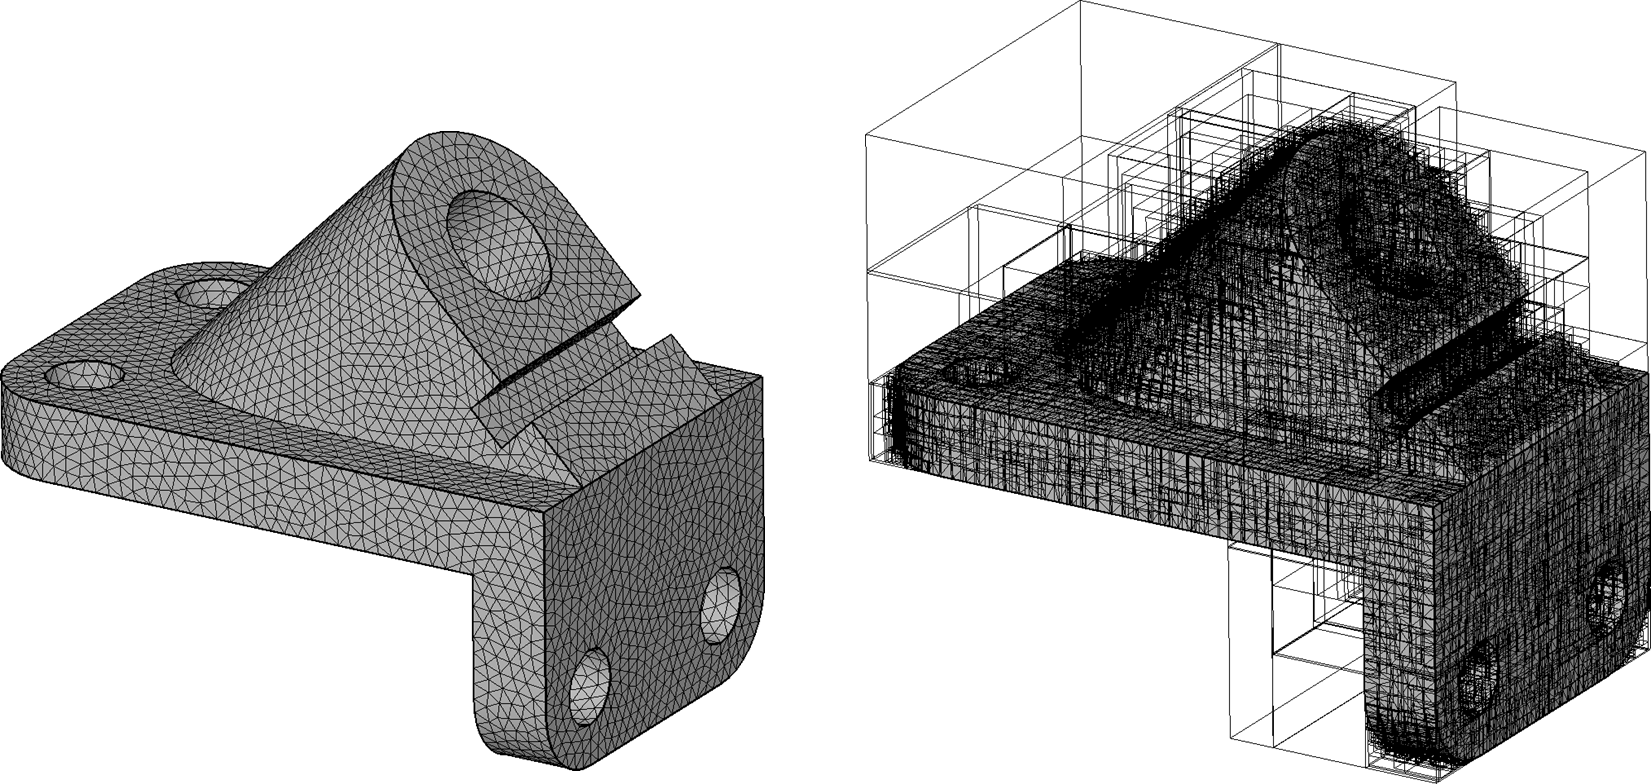
\includegraphics[width=1.0\textwidth]{AABB_tree/anchor}
    \end{ccTexOnly}
    \begin{ccHtmlOnly}
        <img width="99%" border=0 src="./anchor.png"><P>
    \end{ccHtmlOnly}
    \begin{figure}[h]
        \caption{AABB tree.
                 Left: surface triangle mesh of a mechanical part.
                 Right: AABB tree constructed.}
    \end{figure}
\end{center}
